\section{Aufbau und Versuchsdurchführung}

Untersucht wird die mittelere Schicht eines Würfels, der sich insgesamt aus 3x3x3 Elementarwürfeln zusammensetzt; somit wird eine 3x3 Ebene untersucht.
Abbildung ????? zeigt, die ausgewählten Projektionsrichtungen der Messreihen.
Insgesamt wird der Würfel aus 12 Richtungen bestrahlt.





Ein Foto des Versuchsaufbaus in ist Abbildung $\ref{fig:aufbau}$ zu sehen.
\begin{figure}[H]
  \centering
  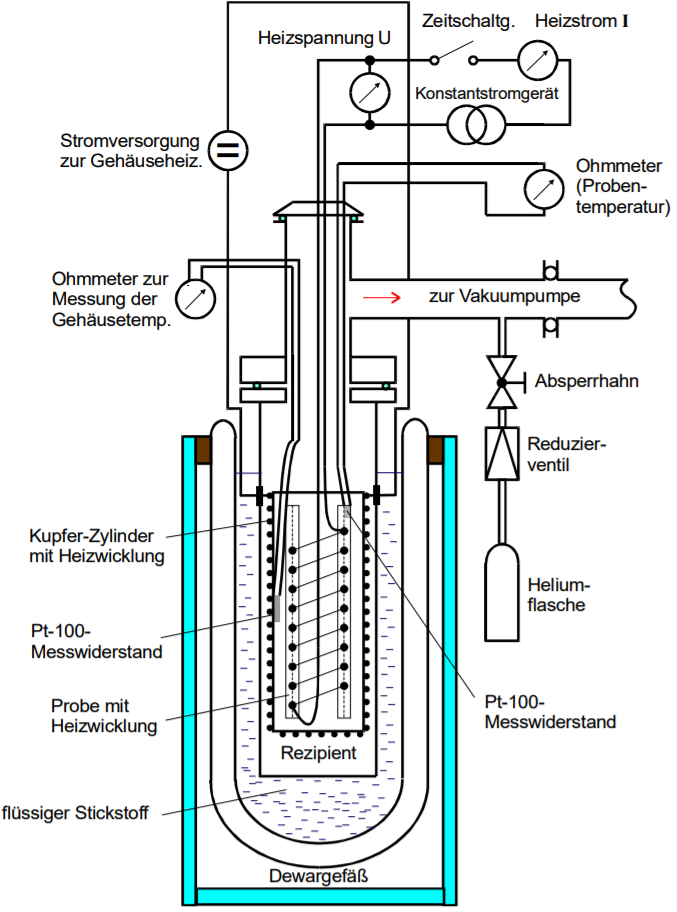
\includegraphics[width=0.8\textwidth]{Bilder/aufbau.png}
  \caption{Aufbau des Experiments.\cite{anleitung}}
  \label{fig:aufbau}
\end{figure}

Die $\gamma$-Strahlungsquelle ist fest im Aufbau installiert. Um die Strahlung möglichst parallel auf den Würfel treffen zu lassen, wird direkt vor der Quelle die Strahlung durch ein
kleines Loch in einer Bleiplatte abgeschirmt und somit kollimiert.
Im Lauf des Strahles ist eine Möglichkeit gegeben, den Würfel beweglich zu platzieren.
Nach Abschirmung durch den Würfel trifft die verbleibende Strahlung auf einen Szintillationsdetektor.
Dieser besteht aus einem anorganischen Szintillator und einem Photomultiplier.
Durch die Bestrahlung wird der Szintillator angeregt und sendet im gleichen Verhältnis zu den eintreffenden Photonen, Lichtblitze aus.


Hierbei wird
